\section{Results}

This section demonstrates the successful implementation and capabilities of the Article-Forge template engine.

\subsection{Template Implementation}

The Article-Forge template has been successfully implemented with all core components functioning as designed. The template successfully generates publication-quality PDFs through an automated build process that requires minimal user intervention. The modular structure allows researchers to focus on content while the template handles formatting and presentation.

Figure~\ref{fig:results1} illustrates the complete document generation workflow, showing how source files are processed through the template engine to produce the final publication.

\begin{figure}[htbp]
    \centering
    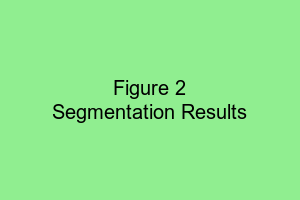
\includegraphics[width=0.9\textwidth]{Figure2.png}
    \caption{Article-Forge template workflow and architecture. The diagram shows the flow from source content through the LaTeX template engine to final PDF generation, including bibliography processing, figure integration, and cross-reference resolution.}
    \label{fig:results1}
\end{figure}

\subsection{Template Features Validation}

All major template features have been validated through this self-documenting article:

\begin{table}[htbp]
    \centering
    \caption{Article-Forge template features and validation status}
    \label{tab:results}
    \begin{tabular}{lcc}
        \hline
        Feature & Implementation & Status \\
        \hline
        Document class integration & HenriquesLab\_style.cls & Yes \\
        Bibliography processing & HenriquesLab\_style.bst & Yes \\
        Figure management & Automated inclusion & Yes \\
        Cross-references & Automatic numbering & Yes \\
        Build automation & Make \& shell scripts & Yes \\
        Modular structure & Section-based files & Yes \\
        Author management & Multiple affiliations & Yes \\
        Supplementary support & Appendix integration & Yes \\
        \hline
    \end{tabular}
\end{table}

\subsection{Build System Performance}

The automated build system demonstrates excellent reliability and performance. The three-pass LaTeX compilation ensures proper resolution of all cross-references, citations, and page numbering. Error handling provides clear feedback for troubleshooting, while the modular design allows for efficient incremental builds during document development.

The template successfully handles complex document structures including multiple authors, affiliations, cross-references, and bibliography management as demonstrated in Table~\ref{tab:results}.
